% Define document class
\documentclass[twocolumn]{aastex631}
\usepackage{showyourwork}

\usepackage{tikz}
\usetikzlibrary{positioning}
\usetikzlibrary{shapes}
\usetikzlibrary{fit}

\newcommand{\comment}[1]{}

% note command for inline notes
\newcommand{\note}[1]{\textsf{\textcolor{red}{#1}}}
% command to note a missing citation
\newcommand{\needscite}{\note{[needs citation]}}

% some commonly used math expressions
\newcommand{\px}{p^{}_{X}}
\newcommand{\pu}{p^{}_{U}}
\newcommand{\R}{\mathbb{R}}

\shorttitle{Modeling Galaxy Catalogues with Normalizing Flows}
\shortauthors{Crenshaw et al.}

% Begin!
\begin{document}

% Title
\title{Statistical Modeling of Galaxy Catalogues with Normalizing Flows}

% Author list
\correspondingauthor{John Franklin Crenshaw}
\email{jfc20@uw.edu}

\author[0000-0002-2495-3514]{John Franklin Crenshaw}
\affiliation{DIRAC Institute and Department of Physics, University of Washington, Seattle, WA 98195, USA}

\author{J. Bryce Kalmbach}

\author{Alexander Gagliano}

\author{Alex Malz}

\author{Sam Schmidt}

\author{Francois Lanusse}

\collaboration{99}{(The LSST Dark Energy Science Collaboration)}

% Abstract
\begin{abstract}
    Normalizing flows are useful for modeling high-dimensional probability distributions.
    We give some background and introduce PZFlow, a Python package for statistical modeling of tabular data.
    We demonstrate via modeling photometry and redshifts for a galaxy catalog, and estimate photo-z posteriors.
    \end{abstract}

% Main body with filler text
\section{Introduction}
\label{sec:intro}

Astronomical data represent realizations of complex probability distributions.
Need to write more here.

While direct access to the probability distributions that characterize our data is usually impossible, machine learning provides powerful tools to learn these distributions from samples thereof.
Generative Adversarial Networks (GANs; \needscite) and Variational Autoencoders (VAEs; \needscite) are two popular methods that provide generative models trained on samples.
However, neither of these methods allow exact evaluation of probability densities.

Normalizing flows are a deep learning tool for density estimation and generative modeling that allow efficient sampling and exact likelihood calculation.
The ability to generate samples from a probability distribution with respect to which you can calculate exact likelihoods is very powerful for generative modeling, as you can provide a notion of ``true'' posteriors over sample properties when simulating new data.
For example, when simulating galaxy catalogs for photometric redshift (photo-z) estimation, you can calculate the ``true'' redshift posterior for each galaxy.
This is useful for ...

To facilitate the statistical modeling of galaxy catalogs and other astronomical data sets, we have developed PZFlow, a normalizing flow package for python.
With relatively little tuning required by the user, PZFlow can provide a generative model for any tabular data, including continuous and discrete variables, and variables with Euclidean or periodic topology.
In addition to generative modeling, PZFlow can calculate posteriors over any columns in your data set, and can convolve errors and marginalize over missing columns while training the model or calculating posteriors for samples.

\note{[need to work in citations to Francois' paper on Deep Generative Models for Galaxy Image Sims, and any other examples of normalizing flows in the astronomy literature.]}

Describe outline of the paper\dots

Mention PZFlow and note that all of the NFs in this paper were created using it.

Maybe mention ShowYourWork and how the scripts and data are all available at the links in the paper.


\section{Normalizing Flows}
\label{sec:nf}

\begin{figure*}[t!]
    \script{plot_two_moons.py}
    \begin{centering}
        \includegraphics{figures/twomoons_example.pdf}
        \caption{
            A normalizing flow demonstrated on the two moons data set from \texttt{scikit-learn}.
            The two moons data on the left is mapped onto a two dimensional uniform distribution by the bijection $f$.
            The data are colored by quadrant to visualize their image in the latent space.
            You can sample the data distribution by sampling from the uniform distribution, and using $f^{-1}$ to map the back to the data space.
        }
        \label{fig:two-moons}
    \end{centering}
\end{figure*}

Normalizing flows model complex, high-dimensional probability distributions by learning a mapping from the data distribution to a tractable latent distribution\footnote{Some of the machine learning literature defines the mapping in the opposite direction.}.
Often the latent distribution is a standard Normal distribution, and so the mapping ``normalizes'' the data, hence the name ``noramlizing flow''.
This mapping allows us to sample and evaluate densities using the latent distribution, rather than the unknown data distribution.

Assume we have a differentiable function $f$ that maps samples $x$ from the data distribution $\px$ onto samples $u$ from the latent distribution $\pu$.
Using the change of variables formula, we can evaluate the probability density of the data:
\begin{align}
    \px(x) = \pu(u=f(x)) \, |\det \nabla f(x)|,
    \label{eq:px}
\end{align}
where $\nabla f(x)$ is the Jacobian of $f$ evaluated at $x$.
In words, computing the density $\px(x)$ is accomplished by mapping $x$ to the latent distribution, calculating its density there, and multiplying by the associated Jacobian determinant, which accounts for how the function $f$ distorts volume elements of the space.

If we further assume that is invertible, we can sample from the data distribution by appling $f^{-1}$ to samples from the latent distribution:
\begin{align}
    x = f^{-1}(u) \quad \text{where} \quad u \sim \pu.
\end{align}

Figure \ref{fig:two-moons} shows an example of a normalizing flow that transforms the \texttt{scikit-learn} two moons distribution into a uniform distribution.
The data points are colored by quadrant to visualize their image under the bijection $f$.

The following sections discuss how to build a normalizing flow to model data with various features.
Section \ref{sec:bijections} discusses the bijection $f$ and introduces the building blocks from which our bijections will be built;
Section \ref{sec:latent} discusses how to choose an appropriate latent distribution for your data;
Section \ref{sec:conditional} describe how to condition a normalizing flow on some conditional variables;
Section \ref{sec:periodic} explains how to model data with periodic topology;
finally Section \ref{sec:discrete} explains how to model data with discrete variables.


\subsection{Designing a bijection}
\label{sec:bijections}

The bijection of a normalizing flow must be powerful enough to model complex relationships in data, while simultaneously possessing an efficiently computable Jacobian determinant.
This latter constraint is the primary difficulty in designing a normalizing flow.
The most popular strategy for achieving these requirements is to exploit the fact that a composition of bijections is also bijective.
By chaining together multiple less-expressive bijections whose Jacobians are efficiently computable, a composite bijections can be constructed that meets our requirements:
\begin{align}
    f &= \dots \circ f_3 \circ f_2 \circ f_1.
\end{align}
The overall Jacobian determinant can be efficiently calculated using the chain rule.

There is an extensive literature on constructing these sub-bijections (see \citealt{kobyzev2020} for a review).
Some bijections are specialized to be particularly efficient at either density estimation or sampling, but for many science cases, we wish to do both.
For this reason, we will focus on Rational-Quadratic Rolling Spline Couplings (RQ-RSCs), which achieve state-of-the-art performance, while being efficient with both tasks \citep{durkan2019}.

\subsubsection{Rational-Quadratic Rolling Spline Couplings}
\label{sec:rq-rsc}

\begin{figure}
    \centering
    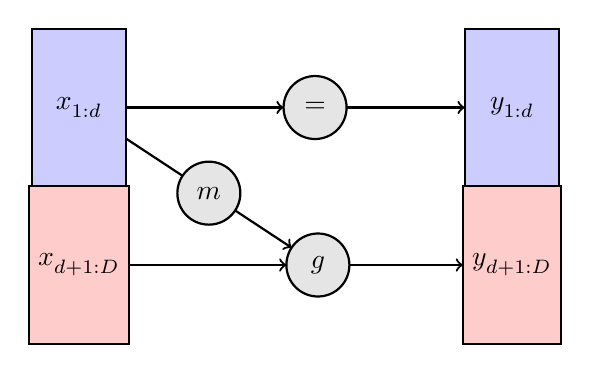
\begin{tikzpicture}[thick, outer sep=0]
        \node [draw, rectangle, minimum height=2cm, minimum width=1.2cm, fill=blue!20] (1) {$x^{}_{1:d}$};
        \node [draw, rectangle, minimum height=2cm, minimum width=1.2cm, fill=red!20, below = 0 of 1] (2) {$x^{}_{d+1:D}$};
        \node [draw, circle, minimum size=8mm, fill=gray!20, right = 2cm of 1] (3) {$=$};
        \node [draw, circle, minimum size=8mm, fill=gray!20, right = 2cm of 2] (4) {$g$};
        \node [draw, rectangle, minimum height=2cm, minimum width=1.2cm, fill=blue!20, right = 1.5cm of 3] (5) {$y^{}_{1:d}$};
        \node [draw, rectangle, minimum height=2cm, minimum width=1.2cm, fill=red!20, below = 0 of 5] (6) {$y^{}_{d+1:D}$};
        \draw[->] (1) -- (3);
        \draw[->] (2) -- (4);
        \draw[->] (3) -- (5);
        \draw[->] (4) -- (6);
        \draw[->] (1) -- (4) node [midway, draw, circle, fill=white, minimum size=8mm, fill=gray!20] {$m$};
    \end{tikzpicture}
    \caption{
    Diagram of a coupling layer.
    The first partition, $x^{}_{1:d}$, is passed through the layer unchanged.
    The second partition, $x^{}_{d+1:D}$, is transformed by the coupling law $g$, which is parameterized by the coupling function $m$ applied to the first partition.
    }
    \label{fig:coupling}
\end{figure}

RQ-RSCs are based on coupling layers \citep{dinh2015, dinh2017}.
A coupling layer partitions the data, $x \in \R^D$, into two sets, $x_{1:d}$ and $x_{d+1:D}$.
The first set is then used to transform the second set:
\begin{align}
    \begin{split}
    y^{}_{1:d} &= x^{}_{1:d} \\
    y^{}_{d+1:D} &= g(x^{}_{d+1:D}; m(x^{}_{1:d})),
    \end{split}
\end{align}
where $g : \R^{D-d} \times \R^d \to \R^{D-d}$ is an invertible \emph{coupling law}, and $m$ is a \emph{coupling function} defined on $\R^d$.
This is illustrated in Figure \ref{fig:coupling}.
The advantage of this structure is that the Jacobian is triangular,
\begin{align}
    \frac{\partial y}{\partial x} =
    \begin{pmatrix}
         I_d & 0 \\
         \frac{\partial y^{}_{d+1:D}}{\partial x^{}_{1:d}}
         & \frac{\partial y^{}_{d+1:D}}{\partial x^{}_{d+1:D}}
    \end{pmatrix},
\end{align}
and in particular, the Jacobian determinant is
\begin{align}
    \det \frac{\partial y}{\partial x} = \det \frac{\partial y^{}_{d+1:D}}{\partial x^{}_{d+1:D}}.
\end{align}
Furthermore, the inverse can be calculated as
\begin{align}
    \begin{split}
    x^{}_{1:d} &= y^{}_{1:d} \\
    x^{}_{d+1:D} &= g^{-1}(y^{}_{d+1:D}; m(x^{}_{1:d})),
    \end{split}
\end{align}
Notice that neither inverting a coupling layer nor calculating the Jacobian determinant requires inverting or taking derivatives of the coupling function $m$, which can thus be arbitrarily complex.

The obvious limitation of a coupling later is that only a subset of the data variables are transformed.
This is overcome by stacking multiple coupling layers in succession, and switching which variables belong to which partition.
In practice, this is achieved by interspersing coupling layers with bijections that shuffle the dimensions of $x$.
These shuffling bijections are trivially inverted and have a Jacobian determinant of one.

There are a variety of different coupling laws one can use.
One particularly expressive choice is a Rational-Quadratic Neural Spline Coupling (RQ-NSC; \citealt{durkan2019}).
As the name suggests, the \emph{coupling law} for RQ-NSCs is a set of rational-quadratic splines and the \emph{coupling function} is a neural network.
RQ-NSCs define a spline $g_i: [-B, B] \subset \R \to [-B, B]$ for each dimension $i$ of $x_{d+1:D}$, where $g_i$ is a piecewise combination of $K$ segments, and each segment is a rational-quadratic function.
The positions and derivatives of the knots that parameterize the splines are calculated from $x_{1:d}$ by a neural network.

RQ-NSCs are state-of-the-art for efficient sampling and density estimation \citep{kobyzev2020}, and are flexible enough to model complex distributions with multiple discontinuities and hundreds of modes.
In addition, they are easily adaptable for flows with periodic topology (Section \ref{sec:periodic}).
For more details, see \citet{durkan2019}.

In this work, we introduce a simple extension of RQ-NSCs, which we name Rational-Quadratic Rolling Spline Couplings (RQ-RSCs).
An RQ-RSC models $D$ dimensional data by stacking $D$ RQ-NSC layers (with $d=D-1$), each followed by a Rolling layer.
A Rolling layer shifts the dimensions of $x$ by one place:
\begin{align}
    \mathrm{Roll}: [x_1, \dots , x_{D-1}, x_D] \to [x_D, x_1, \dots , x_{D-1}].
\end{align}
In other words, RQ-RSCs individually transform each of the $D$ dimensions of $x$ as a function of the other $D-1$ dimensions.
In the limit of high spline resolution (i.e. $K \to \infty$), RQ-RSCs can model any differentiable, monotonic function on $[-B, B]^D$ and can thus model arbitrarily complex distributions in this region.
In practice, we find very good performance for diverse data sets with much smaller $K$.

Note that you can also specify a different value of $K$ for each of the $D$ spline layers in order to individually control the resolution of each dimension.

\subsubsection{Data processing bijections}
\label{sec:data-processing}

While RQ-RSCs perform the heavy lifting of mapping the data distribution $\px$ onto the latent distribution $\pu$, it is also convenient to define other bijections that perform useful operations such as pre- and post-processing.
We name these \emph{data processing bijections}.

For example, RQ-RSCs (and the RQ-NSCs on which they are based) are defined on the domain [-B, B], and thus will not transform samples outside this range.
It is therefore useful to define a \emph{Shift Bounds} bijection, which shifts the original range of each dimension to match the domain of the splines.
Note that this shift must be set at training time, with the assumption that future test data will lie within the same bounds\footnote{This bijection may be poorly suited to data with large outliers. In that case, more care should be taken in designing a bijection that maps the data onto the range of the splines.}.
You can choose a range wider than that covered by the training set if you wish to allow the flow to sample outside the range of the training set.

\note{Discuss the Inverse Softplus Bijection here! If I use it below. Not sure if I will...}

For an example of building an application-specific data processing bijection, see the \emph{Color Transform} bijection defined in Section \ref{sec:fwd-model}, which maps galaxy magnitudes to galaxy colors.
See section \ref{sec:discrete} for data processing bijections, which enable the flow to model discrete data.

Instead of using these data processing bijections, you can of course manually pre-process the data before evaluating densities and post-process samples drawn from the normalizing flow.
However, by building pre- and post-processing directly into the bijection, you remove these extra steps from the workflow.
This reduces the complexity of working with the normalizing flow and ensures that the flow always ``remembers'' how to correctly perform these pre- and post-processing steps.


\subsection{Choosing a latent distribution}

\note{
Discuss latent distributions here.
Note that most applications use a Normal Distribution, but since the splines have a compact domain, we need to choose a latent distribution with compact support, or else we might generate strange outliers when sampling from the flow.
Some text for this might already be in the creation module draft.
}


\subsection{Conditional flows}
\label{sec:conditional}

The bijectors and latent distributions discussed above can be easily adapted to directly learn conditional probability distributions:
you only need to make the replacement $f(x) \to f(x;y)$, where $y$ is a vector of conditions \citep{winkler2019}.
In practice, as the bijection $f$ is parameterized by a neural network, this can be simply achieved by appending the vector $y$ to the neural network's input.

While $p(x|y)$ is technically encoded within $p(x,y)$, which can be learned with a regular normalizing flow, directly modeling $p(x|y)$ with a conditional flow has a few benefits.
Training is typically faster, since the latent distribution has a smaller number of dimensions.
You can also draw samples of $x$ at fixed values of the conditions $y$, and you can calculate $p(x|y)$ without having to numerically calculate and divide by $p(y)$, which can be computationally expensive.

\subsection{Flows with periodic topology}
\label{sec:periodic}

The flows we have considered so far model data that live in $\R^n$.
This assumption is insufficient for modeling variables from spaces with non-Euclidean topology, e.g. positions on the sky.
While progress has been made on building flows for general topologies (e.g. \citealt{gemici2016} and \citealt{falorsi2019}), we will focus on building flows on the sphere, $S^2$, as this is the case most relevant in astronomy.
We will see that by carefully choosing the latent space, we can construct flows with periodic topology with minimal additional effort \citep{rezende2020}.

Positions on the sphere are specified by two angles\footnote{
We use the physicists' convention where $\theta$ and $\phi$ are the zenith and azimuthal angles, respectively.
},
$\theta$ and $\phi$, the latter of which is periodic.
By mapping $\theta$ to $\cos\theta$, we map the sphere to a cylinder\footnote{
This map can be explicitly constructed via an embedding in $\R^3$.
Technically, the map is not defined for $\theta \in \{0, \pi\}$, however as this set has zero measure, it can be safely ignored.}:
$S^2 \to [-1,1] \times S^1$ (i.e. the Cartesian product of an interval and a circle).
In other words, we can transform $\cos\theta$ with a Euclidean flow, as long as we ensure that the flow bounds samples to the range $[-1, 1]$.
However, the $S^1$ piece, $\phi$, has a periodic topology and must be handled more carefully.

First, we will address transformations of $\cos\theta$.
The only constraint we must impose is that samples of $\cos\theta$ must lie in the range $[-1, 1]$.
Fortunately, RQ-NSCs are bounded, mapping a range in $u$ to the same range in $x$.
Thus, if we pick a latent distribution with compact support in $[-1, 1]$, samples of $\cos\theta$ are guaranteed to lie in the same range, as long as we set the range of the RQ-NSC $B$ = 1.

Next we will address transformations of $\phi$.
For $f$ to be a valid diffeomorphism on the circle, $S^1$, it is sufficient that $f$ obey the following constraints:
\begin{align}
    f(0) &= 0 \\
    f(2\pi) &= 2\pi \\
    \nabla f(0) &= \nabla f(2\pi) \label{eq:df=df} \\
    \nabla f(\phi) &> 0.
\end{align}
The first two constraints ensure continuity of $f$ by designating $\phi=0$ as a fixed point, and the third constraint ensures continuity of $\nabla f$ at that fixed point.
While the designation of $\phi=0$ as a fixed point is an unnecessary restriction on $f$, any diffeomorphism on the circle has at least one fixed point up to a phase change, and so this restriction does not actually restrict the expressiveness of $f$.
The fourth restriction ensures monotonicity, which guarantees invertibility.

If we make the phase change $\phi \to \phi - \pi$ so that our angles $\phi \in [-\pi, \pi]$, a RQ-NSC with $B=\pi$ automatically fulfills all four constraints.
In fact, regular RQ-NSC's impose the further condition
\begin{align}
    \nabla f(-\pi) = \nabla f(\pi) = 1 \label{eq:df=1}
\end{align}
to match an identity transform for inputs outside of the range $[-\pi, \pi]$.
By choosing a latent distribution with compact support in the range $[-\pi, \pi]$, we ensure that no samples will lie outside the range of the splines, and so we can relax the boundary condition of Equation \ref{eq:df=1} in favor of the boundary condition in Equation \ref{eq:df=df}.
Spline transforms with this relaxed boundary condition are named \emph{Circular Splines} by \citet{rezende2020}.

See Figure \ref{fig:sphere} for an example of circular splines used to model the population density of the Earth \note{cite the data set here}.
The angles are shifted so that $\phi=\pm \pi$ corresponds to the Prime Meridian.
You can see that the circular splines have no problem with smoothly modeling the data around this discontinuity in $\phi$.

The circular spline construction above is easily generalized to n-spheres and n-tori: $S^n \to [-1, 1]^{n-1} \times S^1$ and $T^n \to (S^1)^n$ (see \citealt{rezende2020} for more details).
We can model the joint distribution of periodic and non-periodic variables with RQ-RSCs simply by choosing appropriate bounds $B$ for each dimension, and by swapping boundary condition \ref{eq:df=1} for condition \ref{eq:df=df} for any periodic dimensions.


\subsection{Modeling discrete variables}
\label{sec:discrete}

In addition to the continuous variables described above, normalizing flows can also be used to model discrete variables.
This can be achieved by ``dequantizing'' the discrete dimensions of the data, which can then be mapped onto continuous latent distributions using regular continuous bijectors.
Dequantization consists of adding some kind of continuous noise to the discrete dimensions, transforming them into continuous dimensions.
When sampling from the flow, you simply do the opposite, and ``quantize'' the discrete dimensions after applying all of the regular bijections, mapping the noisy, continuous variables onto their discrete counterparts.

A common method for dequantization is uniform dequantization, in which random uniform noise in the range (0, 1) is added to the discrete dimensions.
The corresponding quantization applied while sampling from the flow consists of applying the floor function to the dequantized dimensions, mapping these samples onto the nearest integer less than the sampled value.
More sophisticated dequantization schemes use variational inference or even another normalizing flow to determine the noise distributions, which improves results by smoothing the discontinuities between neighboring discrete values.
See \citet{ho2019} \citet{hoogeboom2020} for more details.

While the dequantizers are not technically bijections, they can be treated as data processing bijections and be chained together with the other bijectors in your normalizing flow.

\note{Try to get the discrete example working again! Add a figure here.}


\section{PZFlow}
\label{sec:pzflow}

PZFlow is a Python package for building normalizing flows, with a focus on easy high-performance modeling of high-dimensional tabular data.
Data is handled in Pandas DataFrames \citep{pandas}, while the normalizing flows are implemented in Jax \citep{jax}, which allows for efficient, parallelizable, GPU-enabled calculations for very large data sets.
The code is easily installable for the Python Package Index\footnote{\url{https://pypi.org/project/pzflow/}} (PyPI) and is hosted on Github,\footnote{\url{https://github.com/jfcrenshaw/pzflow}}.
The documentation\footnote{\note{URL}} includes tutorial notebooks covering all of the features demonstrated in this paper.

PZFlow is a package for building normalizing flows in Python, with a focus on high-performance out-of-the-box modeling of high dimensional tabular data.
Data is handled in Pandas DataFrames \citep{pandas} while the normalizing flows are implemented in Jax \citep{jax}, which allows efficient, parallelizable, GPU-enabled calculations for very large data sets.
The code is easily installable from the Python Package Index\footnote{\url{https://pypi.org/project/pzflow/}} (PyPI) and is hosted on Github,\footnote{\url{https://github.com/jfcrenshaw/pzflow}} including several tutorial notebooks.

The rest of this paper will demonstrate using PZFlow for the statistical modeling of galaxy catalogs.
Section \ref{sec:galaxy-catalog} uses PZFlow to forward model a photometric catalog, including spectroscopic redshifts, Rubin photometry, ``true'' photo-z posteriors, ellipticities, and sizes.
Section \ref{sec:photo-z} uses PZFlow for photo-z estimation, demonstrating the power of PZFlow as a density estimator, including numerous useful features for photo-z estimation.

In addition to the examples in this paper, PZFlow has already being used in various other projects:
\begin{itemize}
    \item \needscite used PZFlow to build a metric for observing strategy optimization based on information theory;
    \item \needscite used PZFlow to forward model galaxy data with true redshift posteriors in order to evaluate the impact of survey incompleteness and spec-z errors on photo-z estimation;
    \item \needscite used PZFlow to smooth high-redshift artifacts in simulations of supernova host galaxy simulations.
\end{itemize}


\section{Forward Modeling a Galaxy Catalog}
\label{sec:galaxy-catalog}

In this section, we apply PZFlow to forward model a photometric galaxy catalog for the Rubin Observatory.
The advantage of using a catalog generated from a normalizing flow is that we have direct access to the exact distribution from which the data is drawn, enabling us to calculate truth values for derived statistical products, such as the true photo-z redshift posterior for each galaxy.

In Section \ref{sec:fwd-model} we construct a normalizing flow to model the galaxy redshifts and photometry.
In Section \note{LABEL}, we calculate posteriors?
In Section \ref{sec:fwd-model-conditional} we build a conditional flow to add additional properties to the catalog.

\subsection{Forward modeling redshifts and photometry}
\label{sec:fwd-model}

\begin{figure*}[t!]
    \script{plot_main_galaxy_corner.py}
    \begin{centering}
        \includegraphics{figures/main_galaxy_corner.pdf}
        \caption{
            Distribution of the CosmoDC2 test set compared to the distribution learned by PZFlow.
            The close overlap of every pair-wise disttribution demonstrates that PZFlow was able to learn the structure present in CosmoDC2 with high fidelity.
        }
        \label{fig:main-corner}
    \end{centering}
\end{figure*}

To create a generative model of galaxy redshifts and photometry, we use the true redshifts and $ugrizy$ magnitudes from the DESC CosmoDC2 simulation (\needscite).
We selected all galaxies from CosmoDC2 with at most one band beyond the LSST 10-year 5-sigma point source depths.
Of these, we selected $10^6$ galaxies and split them intro training and test sets consisting of 80\% and 20\% of the galaxies, respectively.

For the latent distribution we use a 7 dimensional Uniform distribution over the range $[-5, 5]$.
To map the data onto the latent distribution, we use the following bijection:
\begin{align}
    f = \text{RQ-RSC} \circ \text{Shift Bounds} \circ \text{Color Transform}.
\end{align}
\note{I might add an InverseSoftPlus}
We will explain each layer of the bijection in the order they are applied to the input data.

The first layer of the bijection is a Color Transform.
This bijection converts galaxy magnitudes to colors, but keeps the $i$ band magnitude as a proxy for the apparent luminosity:
\begin{multline}
    \text{Color Transform} : (\text{redshift},\, u,\, g,\, r,\, i,\, z,\, y) \to \\
    (\text{redshift},\, i,\, u-g,\, g-r,\, r-i,\, i-z,\, z-y).
\end{multline}
This layer is useful as galaxy redshifts correlate more directly with galaxy colors than galaxy magnitudes.

The next layer, Shift Bounds, is the data processing bijection defined in Section \ref{sec:data-processing}, which maps the range of the data onto the support of the RQ-RSC.
Note that since Shift Bounds is on the ``other side'' of the Color Transform, we need to map the ranges of the colors $u-g$, $g-r$, etc. onto the support of the splines, instead of the original magnitudes.

The final layer is an RQ-RSC, described in detail in Section \ref{sec:rq-rsc}.
This layer performs the heavy lifting of transforming the data distribution into the uniform latent distribution.
We use $D=7$ layers to transform all 7 dimensions of our data, and set $B=5$ to match the support of the latent distribution.
We use the coupling function (with two hidden layers of 128 neurons) described in \citet{durkan2019}.
We use $K=16$ spline knots.

We trained the normalizing flow for 150 epochs using the Adam optimizer \citep{adam} (with a learning rate of $10^{-3}$, that decreased by a factor of 10 every 50 epochs) to minimize the negative log-likelihood,
\begin{align}
    \mathcal{L} = - \, \mathbb{E}[ \, \log p(x) \, ],
\end{align}
where the expectation is performed over galaxies in the training set and $p(x)$ is defined in Equation \ref{eq:px}.
Training took 7 minutes on a Tesla P100 12GB GPU.

We assess the results by drawing $10^4$ galaxies from the trained flow, and plotting their distribution against  $10^4$ galaxies from the test set (Figure \ref{fig:main-corner}).
We see that the normalizing flow has done an excellent job of reproducing the distribution of DESC DC2, without any unusual artifacts or outliers.
We note that these results were obtained without any extensive hyperparameter search, and that very similar (slightly worse results) are obtained without the \texttt{ColorTransform} bijection, demonstrating the flexibility of the method to adapt to unseen data sets.

With this normalizing flow, we have an efficient CosmoDC2 emulator that produces a smooth distribution of realistic galaxies up to high-redshifts.

To simulate photometric errors, we use the LSST error model of \citet{ivezic2019}, except without the high-SNR assumptions made there (see Appendix B for details).

\subsection{Calculating true posteriors}
\label{sec:true-posteriors}

Since we have direct access to the probability distribution from which the photometry and redshifts are drawn, we can calculate the true redshift posterior for each galaxy: $p(z|m)$ where $m$ is the vector of galaxy magnitudes.
We note that this is not an estimate, like what would be returned by a photo-z estimator, but rather the truth, obtained from the model that generated the photometry and redshifts in the first place.

In addition to calculating the true posterior, $p(z|m)$, we can calculate a true posterior that is consistent with the photometric errors:
\begin{align}
    p(z|m, \sigma_m) = \int p(z|\hat{m}) p(\hat{m}|m, \sigma_m) d\hat{m},
    \label{eq:err-conv}
\end{align}
where $\sigma_m$ is the vector of photometric errors returned by the error model, and $\hat{m}$ are possible noisy observations of the true magnitudes, $m$.
We can evaluate this integral numerically by sampling $\hat{m} \sim p(\hat{m}|m, \sigma_m)$, evaluating $p(z, \hat{m})$ on a redshift grid, and normalizing to obtain $p(z|\hat{m})$.
Averaging $p(z|\hat{m})$ over the samples $\hat{m}$ yields $p(z|m, \sigma_m)$.

We can also marginalize over any missing bands, $n$:
\begin{align}
    p(z|\hat{m}) = \frac{1}{p(\hat{m})} \int p(z, n, \hat{m}) dn,
\end{align}
which can be calculated by evaluating $p(z, n, \hat{m})$ on a grid of $z$ and $n$, summing over $n$ to yield $p(z, \hat{m})$, and normalizing with respect to redshift to yield $p(z|\hat{m})$.
You can once again average over $\hat{m}$ samples to convolve the photometric errors.
You may wish to marginalize over all values of $n$ if the galaxy was not observed in that band.
This might occur, for example, if you include photometry from Euclid, which will not have complete coverage of the LSST catalog \needscite.
You may also wish to marginalize over all values beyond a limiting magnitude if the galaxy was observed, but not detected in that band.
This might occur, for example, in the low wavelength bands of Lyman dropout galaxies observed by LSST.

\note{Figure of the posteriors.}

Figure \ref{fig:posteriors} shows a number of redshift posteriors to visualize the effects of error convolution and band marginalization.
The black posterior is calculated using the true galaxy magnitudes, while the blue posteriors is calculated after adding photometric errors.
Calculating the posterior using the noisy photometry results in a biased posterior.
The orange posterior has had the photometric errors convolved as in Equation \ref{eq:err-conv}.
Convolving the errors de-biases the posterior, but the resultant posterior is broader, reflecting the increase uncertainty due to the photometric errors.
Finally, the green posterior has had the $u$ band marginalized.
This posterior is even broader, with a significant low-redshift tail, demonstrating how the loss of information in the $u$ band translates to a loss of information about the redshift.
\note{WILL NEED TO UPDATE THIS AFTER MAKING THE NEW FIGURE.}

Calculating these posteriors enables direct comparison of true redshift posteriors (consistent with the photometric errors and missing bands) with the redshift posteriors estimated by photo-z estimators.
This allows you to test photo-z estimation on a posterior-per-galaxy basis, which will alleviate the photo-z validation problems discovered by \citet{schmidt2020}.


\subsection{Additional properties with conditional flows}
\label{sec:fwd-model-condtional}

In addition to the galaxy magnitudes and redshifts modeled above, we wish to include other galaxy properties in the catalog, such as galaxy size and ellipticity.
In principle, we could have included these variables in the original normalizing flow.
However, we did not want the true redshift posteriors to be conditioned on these variables, as most photo-z estimators only use galaxy photometry.
Therefore, we will build a second flow that models these additional values conditioned on the galaxy redshift and magnitudes.
Note that while we have only chosen to model these additional two properties, any other values you desire can be similarly modeled.

For the latent distribution, we once more use a Uniform distribution over the range $[-5, 5]$.
For the bijection, we use
\begin{align}
    \begin{split}
        f =& ~ \text{RQ-RSC} \circ \text{Shift Bounds}. \\
    \end{split}
\end{align}
The RQ-RSC acts on the two dimensional space of size and ellipticity, but also takes the galaxy redshift and magnitudes as inputs.
The redshifts and magnitudes are transformed to have zero mean and unit variance before being input to the neural network\footnote{These variables are standard scaled instead of mapped onto the domain [-5, 5], because the neural network that parameterizes the splines has no limit on inputs, unlike the splines themselves, which are limited to the range [-5, 5].} that parameterizes the splines.
Aside from the change in inputs, the RQ-RSC has the same settings as listed for the previous normalizing flow.

The conditional flow is trained for \note{N} epochs using the same loss function and optimizer as before.
\note{is the LR the same?}
We sample a size and ellipticity for each galaxy in the PZFlow catalog created in the previous section (using the true magnitudes), and plot the distribution of these features against the distribution in the test set (Figure \note{N}).
Once again, we see that the normalizing flow does a good job of emulating the CosmoDC2 distribution.

The final simulated catalog consists of $10^4$ galaxies, each with a redshift, $ugrizy$ magnitudes including photometric errors, a true photo-z posterior consistent with the photometric errors, a size, and an ellipticity.
This small catalog was generated for visualization purposes, but the normalizing flows can be used to generate catalogs of arbitrarly large size (see Appendix C on benchmarking PZFlow).


\section{Photometric Redshift Estimation}
\label{sec:photo-z}

\appendix
A. Failed (?) experiments

- CentBeta - harder to train, slower, results aren't better
- convolving Gaussian errors analytically (use the trained flow from above to plot the gradients of the spline or something and show that the necessary assumptions are not valid)

B. LSST Error Model

- Explain how I adapted the LSST Error Model to work for low-SNR galaxies

C. Benchmarking PZFlow


\bibliography{references.bib}


\end{document}
